% \section{Quantitative Implications}

% In this section, we consider the quantitative implications of the model described in Section~\ref{sec:model}. 

 
% \subsection{Calibration strategy}
% \paragraph{Sectors.}
% We process raw flow of funds (FOF) data to arrive at $J=6$ major sectors: household mutual fund holdings, households non-mutual fund holdings, hedge funds, broker-dealers (L130), rest of the world (L133), and hedge funds. 

% To visualize the size of these ultimate sectors, Figure~\ref{fig:sectors} plots the fraction of the U.S. stock market held by each sector from 2012 when hedge fund holdings became available. Figure~\ref{fig:sectors}'s legend reports the average fraction held by each sector. The largest holder is the household sector which holds 17.3\% via mutual funds and 43.3\% through other means. The net largest sectors are foreign investors (``rest of the world'') and pension/insurance sectors which hold 17.5\% and 17.3\%, respectively. Hedge funds and broker-dealers are relatively small and hold 5.8\% and 0.5\%, respectively, consistent with Figure 1 in \cite{koijen2024investors}. 

% \begin{figure}[t]
%     \centering
%     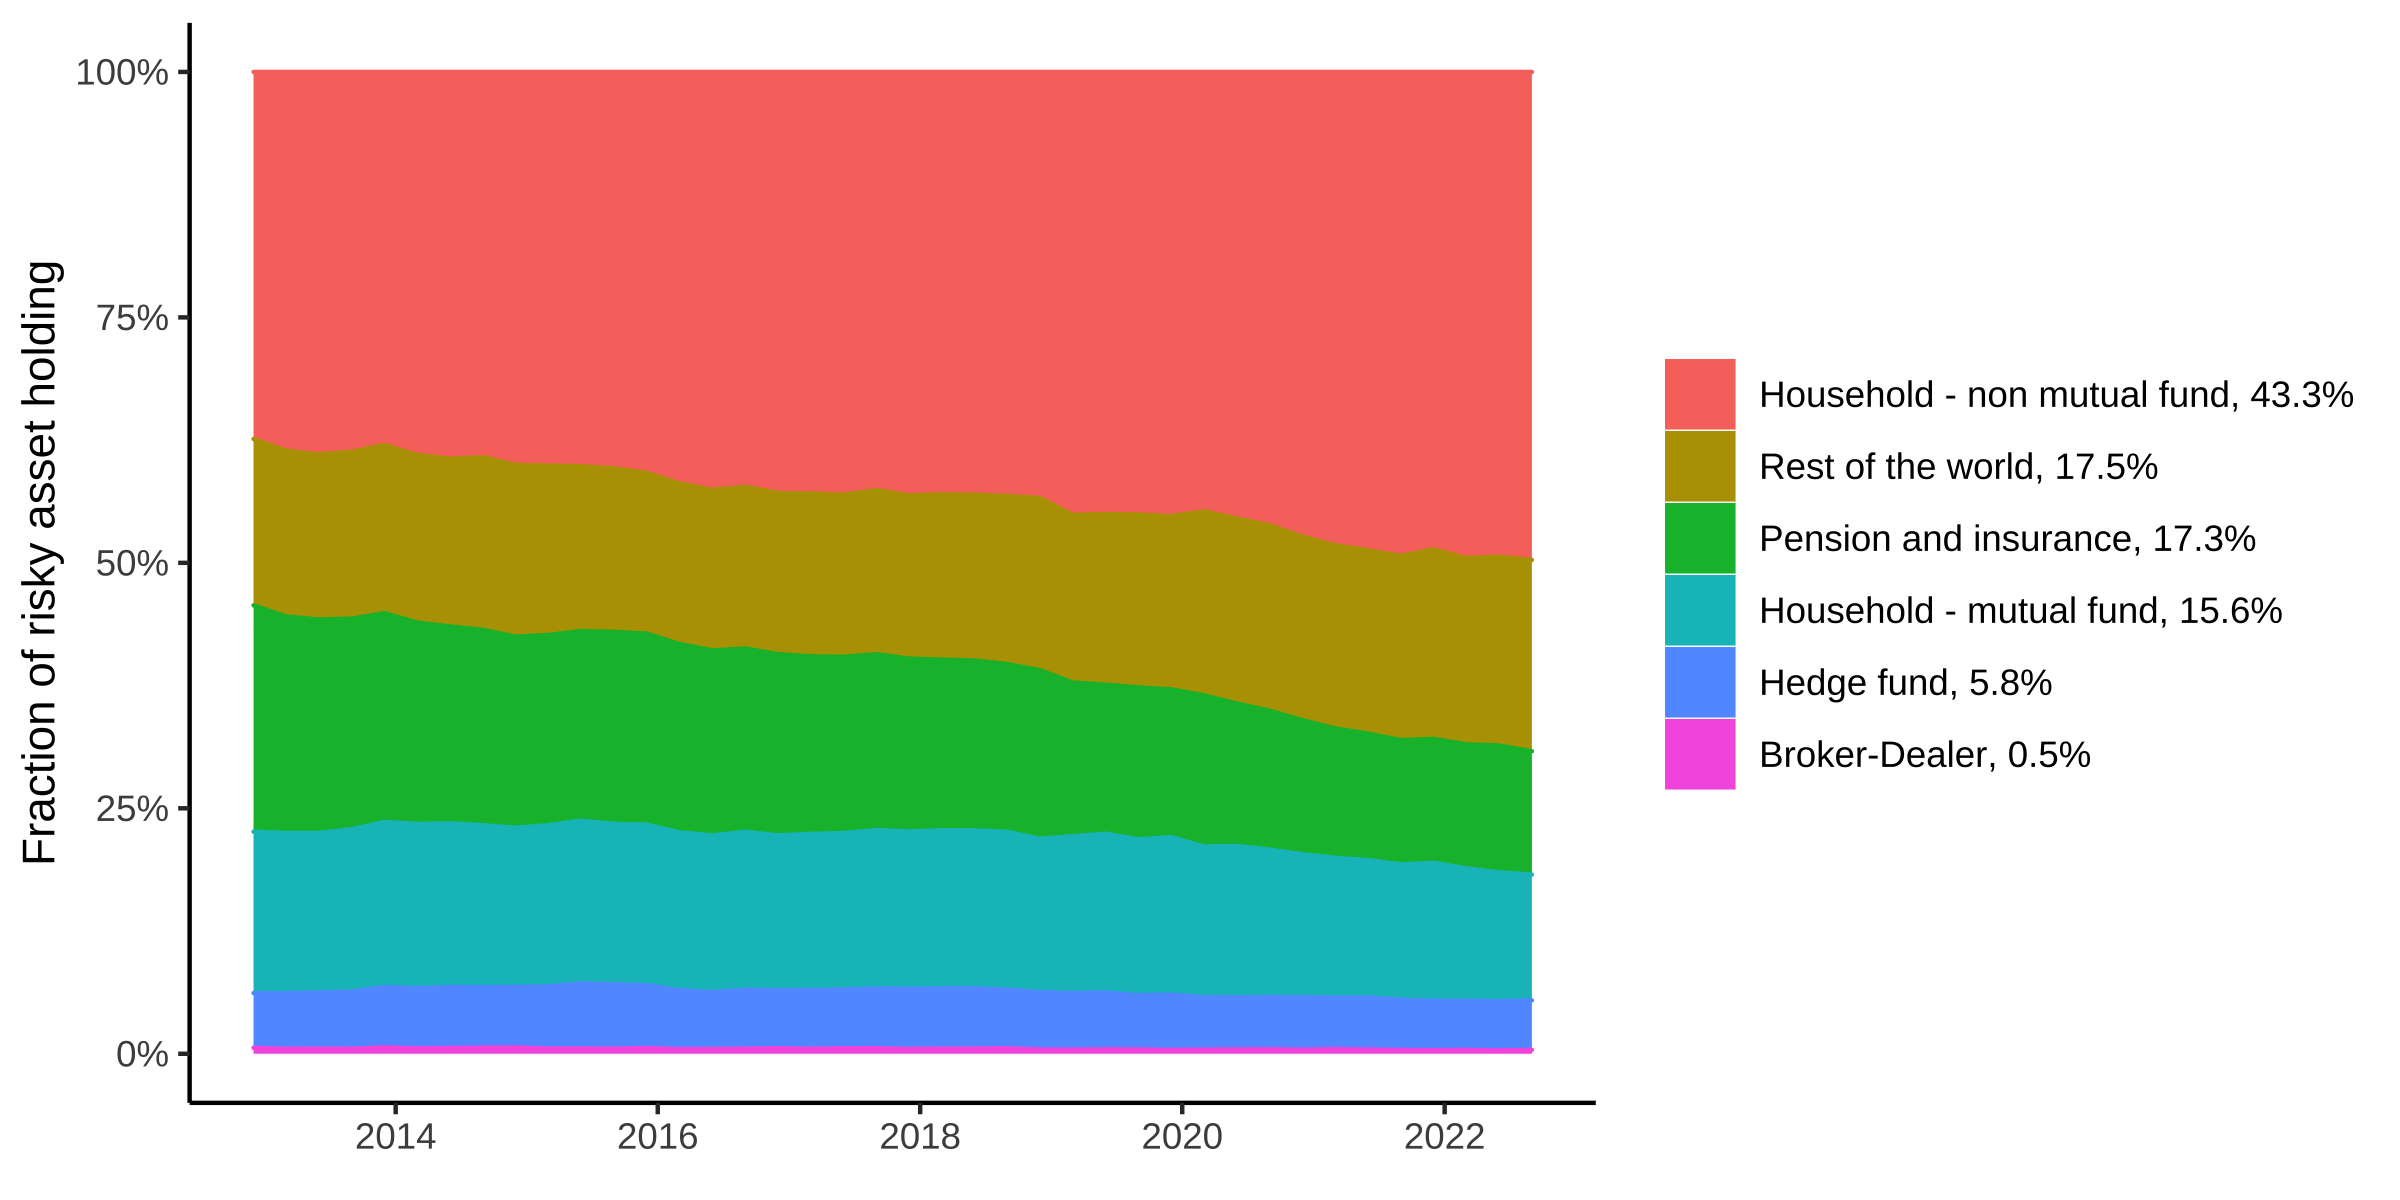
\includegraphics[width=0.9\linewidth]{figures/break_down_of_holdings.png}
%     \caption{Fraction of stock market holding by sectors from 2012 to 2022. The average fraction held is reported in the legend. Source: Flow of Funds.}
%     \label{fig:sectors}
% \end{figure}

% We first drop sectors that have no or minimal investments in the stock market. This includes nonfinancial business (L102), general government (L105), monetary authority (L109), Private depository institutions (L110), money market funds (L121), Government-sponsored enterprises (L125), Agency-and GSE-backed mortgage pools (L126), and Issuers of asset-backed securities (L127), Finance companies (L128), Real estate investment trusts (L129), Holding companies (L131), and Other financial business (L132). We then aggregate sectors that invest in the stock market but are pass-throughs onto the end users' balance sheets. 

% Mutual funds (L122), Closed-end funds (L123), and Exchange-traded funds (L124): we aggregate L123 and L124 onto the household (L101) balance sheet. For mutual fund holdings (L122), FOF provides a detailed breakdown of end investors. We aggregate the non-household holdings onto the respective end investor balance sheets but separately consider the household holdings as a separate sector. 
% We aggregate all defined contribution pensions (Tables L118c, L119c, and L120c) onto household balance sheet. 

% We then separate out the hedge fund sector. Both the household (L101) and foreign (L133) sectors contain hedge funds. Because hedge funds likely behave differently from other sectors, we separate them out. We use Table B.101.f to capture domestic hedge funds and use the hedge fund table in enhanced financial accounts to also capture foreign hedge funds. We consider all hedge funds a single sector, and we subtract their holdings from the household and foreign sectors. Finally, we aggregate together all remaining insurance and pension sectors. This includes property-casualty insurance (L115), life insurance (L116), and defined benefit pension and retirement plans (L118b, L119b, L120b).

% \paragraph{Mass of investors and risk aversion coefficients.}
% We choose $\omega_j$ and $\gamma_j$ for each sector $j$ to match the following moments:
% \begin{itemize}
%     \item 	$\frac{1}{T} \sum_t\frac{Assets_{j,t}}{\sum_i Assets_{i,t}}$, which corresponds to $\frac{1}{T}\frac{\sum_t\omega_jW_{j,t}}{\sum_t\sum_i\omega_iW_{i,t}}$ in the model
%     \item $\{b_j\}_j$ from time-series regressions of
%     \[\text{Risky Asset}_{j,t}=a_j+b_j\left(\sum_j\text{Risky Asset}_{i,t} \right), \]
%     which corresponds in the model to the regression coefficient in the following regression in the model:
%     \[\omega_jW_{j,t}\alpha_{j,t}=a_j+b_j\sum_i\omega_iW_{i,t}\alpha_{i,t}\]
%     \item Only for active sectors $(j=1,2,\ldots,J)$
% \end{itemize}

% \paragraph{Average passive Share $\boldsymbol{\overline{\alpha}}$.}
% There seems to be a big range in the literature from a third to over two thirds:
% \begin{itemize}
%     \item \cite{chinco2024passive} find passive share of 33\%: Each time that a stock gets added to or dropped from an index they ask: ``How much money would have to be tracking that index to explain the enormous burst in closing volume on reconstitution day that we observe in the data?'' 
%     \item \cite{koijen2024investors} find a much larger passive share of 67.2\% in 2016Q4. They use the active share, modified for their application, as a measure of active investment management (\citealp{cremers2009active}).
% \end{itemize}
% We need to find the total passive wealth and divide to get portfolio share.

% \paragraph{Calibrating the Passive Demand Process.}
% Type $j=0$ investors are passive, and their portfolio weight follows and exogenous CIR process in Equation~\eqref{eq:alpha_p_process}, reproduced below:
% \begin{equation*}
%     d \overline{\alpha}_{p,t} = \theta_p (\overline{\alpha} - \overline{\alpha}_{p,t}) dt + \sigma_{p} \sqrt{\overline{\alpha}_{p,t}}\, d Z_t,
% \end{equation*}
% \begin{enumerate}
%     \item Average passive demand ($\overline{\alpha}$): 
%     \begin{itemize}
%         \item Calibrating the average risky asset share of the passive sector is discussed above.
%     \end{itemize}
%     \item Volatility of the passive demand ($\sigma_p$)
%     \begin{itemize}
%         \item Following Appendix D3 of \cite{gabaix2020search}, to measure equity flows, we scale the dollar equity flows for each sector $j$, $\Delta F_{j,t}^\varepsilon$, by the size of the aggregate market in the previous quarter, $\varepsilon_{t-1}$ i.e., $\Delta F_{j,t}^\varepsilon/\varepsilon_{t-1} $.  
%         \item We use indirect inference by matching total flows (the blue line in the left panel of Figure~\ref{fig:facts-vol-flow}). This is our attempt to replicate the red dashed line in Figure D.7 in \cite{gabaix2020search}.
%     \end{itemize}
%     \item Persistence of passive demand ($\theta_p$)
%     \begin{itemize}
%         \item We follow the literature on household portfolio inertia. \cite{brunnermeier2008wealth}, using PSID data, document substantial inertia in households’ portfolios, with very limited or slow rebalancing. This implies that portfolio shares would move with shocks to returns, consistent with the exposure of $\overline{\alpha}_p$ to aggregate shocks. 
%         \item \cite{brunnermeier2008wealth} ``use the information on net purchases or sales of risky assets to construct a variable $\Delta_k\text{Inert}_t$, representing the (counterfactual) change in the liquid risky asset share that the household would have experienced between $t-k$ and $t$ under perfect inertia---that is, if it had not undertaken any purchases or sales of risky assets between $t-k$ and $t$.'' They regress household portfolio weight on inertia ($\Delta_k\text{Inert}_t$), and $k$-period difference in post consumption wealth and major changes in family composition or asset ownership. They find the coefficient on the inertia variable is large, around 0.75, with small standard errors. Taken at face value, it suggests that there is huge inertia. Households' asset allocations seem to fluctuate strongly as a function of in- and outflows, and capital gains and losses, without much rebalancing taking place. 
%         \item Similarly, \cite{parker2023retail} show that the introduction of target-date funds has led to a relatively stable portfolio share, consistent with the evidence in \cite{brunnermeier2008wealth}.
%     \end{itemize}
%     \item Correlation between flow shocks, i.e., innovations in $\overline{\alpha}_p$, and the aggregate shock
%     \begin{itemize}
%         \item We regress quarterly flows, the blue line in the left panel of Figure~\ref{fig:facts-vol-flow}, on the market. The beta coefficient can be used to indirectly get the correlation between flow shocks and aggregate socks.
%     \end{itemize}	
% \end{enumerate}

% Table~\ref{tab:calib} lists the parameter values used in calibrating the model.

% \begin{table}[!t]    \captionsetup{font=normalsize,labelfont=bf,skip=2pt,labelsep=period}
% 	\caption{\textbf{Parameter values}}
% 	\caption*{\footnotesize{This table reports the parameter values used in calibrating the model.}}
%     \vspace{2mm}
%     \label{tab:calib}
%     \centering
%     \resizebox{.65\linewidth}{!}{\begin{tabular}{llc}
	\toprule	
	& Parameter & Choice  \\
	\midrule 
	&\small \emph{Preferences \& distribution}  & \\
	\midrule		
	$\psi$         & EIS & 1.50   \\
	$\gamma_0$     & Risk aversion of passive investors               & 10.86    \\
	$\gamma_j$     & Risk aversion of constrained investors                & 6.15 \\
    $\gamma_j$     & Risk aversion of unconstrained investors                & 25.52 \\ 
	$\rho$         & Effective discount rate                  & 0.01 \\
    $\kappa$       & Agent turnover rate                      & 0.10 \\
    $\omega_0$    & Share of passive agents                & 0.50 \\
    $\omega_1$    & Share of unconstrained agents                & 0.25 \\
	$\omega_2$    & Share of constrained agents                & 0.25 \\
	\midrule 
	& \small \emph{Technology}  & \\
	\midrule 
	$\mu$          & Endowment growth rate                    & 0.018  \\
	$\|\sigma\|$       & Endowment volatility                     & 0.033  \\
    $\|\sigma_s\|$     & Dividend share volatility                & 0.11 \\ 
    $\bar{s}$      & Mean dividend share                      & 0.60 \\ 
    $\kappa_s$     & Mean reversion of dividend share         & 0.09 \\
	$\nu_s$     & Corr. of dividend share and fundamental shock         & 0.30 \\
	\midrule 
	&\small \emph{Passive demand}&  \\
	\midrule
	$\overline{\alpha}$ & Mean &  0.52	\\
    $\theta_p$              & Mean reversion parameter  &  0.75 	\\
    $\sigma_p$             & Passive demand shock exposures &  0.02	\\
    $\nu_p$                  & Corr. of passive demand and fundamental shock & 0.50 \\ 

	\midrule
	& \small \emph{Leverage constraints}  & \\
	\midrule 
	$\overline{\sigma}$ & Tightness of the leverage constraint &  0.11	\\
	\bottomrule
\end{tabular}

%γ_vec=[10., 9.368, 4.925, 3.212, 1.552],
%ψ=2.5,
%ρ_=0.02,
%μ=0.022,
%σ=0.035,
%θp=0.69,
%σp0_=0.1,
%σp1_=0.02,
%σ_hat=0.02,
%κ_=0.05,
%α_=.1,
%ω=0.90713995, 0.02905808, 0.02313385, 0.02031372, 0.02035439}
% \end{table}
% % We calibrate the model with five agents, one passive and four active. Table~\ref{tab:calibration} presents the parameter values. The leverage constraint is occasionally binding: 64\% of the time no one's constraint is binding,
% % 9\% of the time the least risk averse is constrained, 12\% of the time the 2 less risk averse agents are constrained, and 15\% of the time the 3 less risk averse are constrained. 
% % The average price-dividend ratio is 16.06 and its standard deviation is 0.086.
% % \begin{table}[!ht]
% %     \centering
% %     \resizebox{0.7\textwidth}{!}{\begin{tabular}{llc}
	\toprule	
	& Parameter & Choice  \\
	\midrule 
	&\small \emph{Preferences \& distribution}  & \\
	\midrule		
	$\psi$         & EIS & 1.50   \\
	$\gamma_0$     & Risk aversion of passive investors               & 10.86    \\
	$\gamma_j$     & Risk aversion of constrained investors                & 6.15 \\
    $\gamma_j$     & Risk aversion of unconstrained investors                & 25.52 \\ 
	$\rho$         & Effective discount rate                  & 0.01 \\
    $\kappa$       & Agent turnover rate                      & 0.10 \\
    $\omega_0$    & Share of passive agents                & 0.50 \\
    $\omega_1$    & Share of unconstrained agents                & 0.25 \\
	$\omega_2$    & Share of constrained agents                & 0.25 \\
	\midrule 
	& \small \emph{Technology}  & \\
	\midrule 
	$\mu$          & Endowment growth rate                    & 0.018  \\
	$\|\sigma\|$       & Endowment volatility                     & 0.033  \\
    $\|\sigma_s\|$     & Dividend share volatility                & 0.11 \\ 
    $\bar{s}$      & Mean dividend share                      & 0.60 \\ 
    $\kappa_s$     & Mean reversion of dividend share         & 0.09 \\
	$\nu_s$     & Corr. of dividend share and fundamental shock         & 0.30 \\
	\midrule 
	&\small \emph{Passive demand}&  \\
	\midrule
	$\overline{\alpha}$ & Mean &  0.52	\\
    $\theta_p$              & Mean reversion parameter  &  0.75 	\\
    $\sigma_p$             & Passive demand shock exposures &  0.02	\\
    $\nu_p$                  & Corr. of passive demand and fundamental shock & 0.50 \\ 

	\midrule
	& \small \emph{Leverage constraints}  & \\
	\midrule 
	$\overline{\sigma}$ & Tightness of the leverage constraint &  0.11	\\
	\bottomrule
\end{tabular}

%γ_vec=[10., 9.368, 4.925, 3.212, 1.552],
%ψ=2.5,
%ρ_=0.02,
%μ=0.022,
%σ=0.035,
%θp=0.69,
%σp0_=0.1,
%σp1_=0.02,
%σ_hat=0.02,
%κ_=0.05,
%α_=.1,
%ω=0.90713995, 0.02905808, 0.02313385, 0.02031372, 0.02035439}
% %     \caption{Parameter values}
% %     \label{tab:calibration}
% % \end{table}
% % As shown in the left panel of Figure~\ref{fig:price-impact-dist} and consistent with the empirical estimates in \cite{gabaix2020search}, the average price impact is about 5. From the left panel and consistent with the model, the price impact is decreasing in active share $x_a$.

% % \begin{figure}[!ht]
% %     \centering
% %     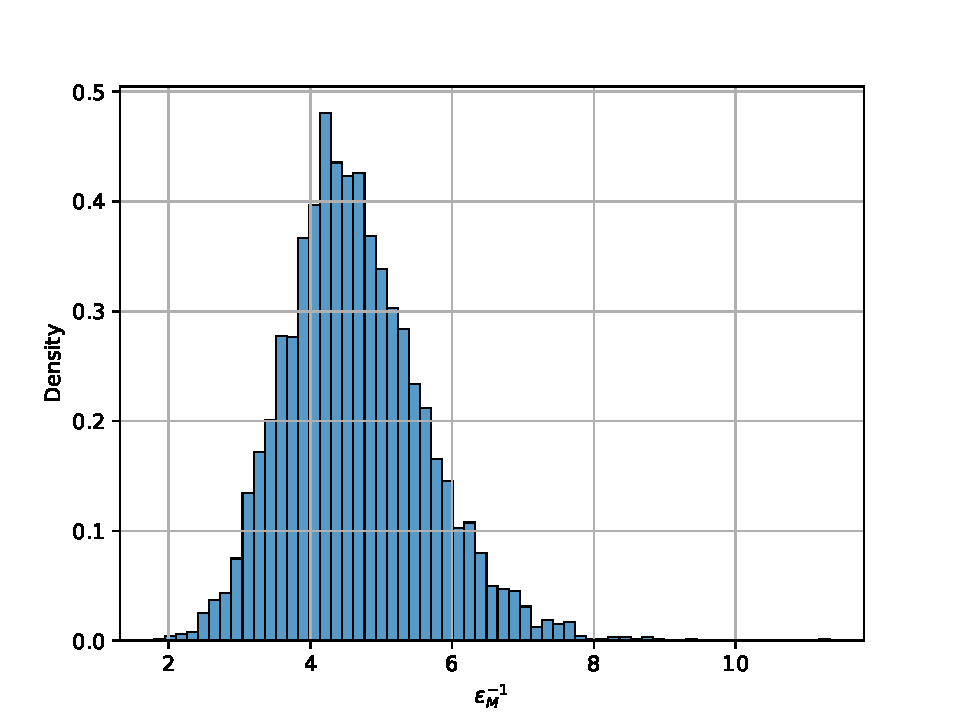
\includegraphics[width=0.49\textwidth]{figures/elasticity.pdf}
% %     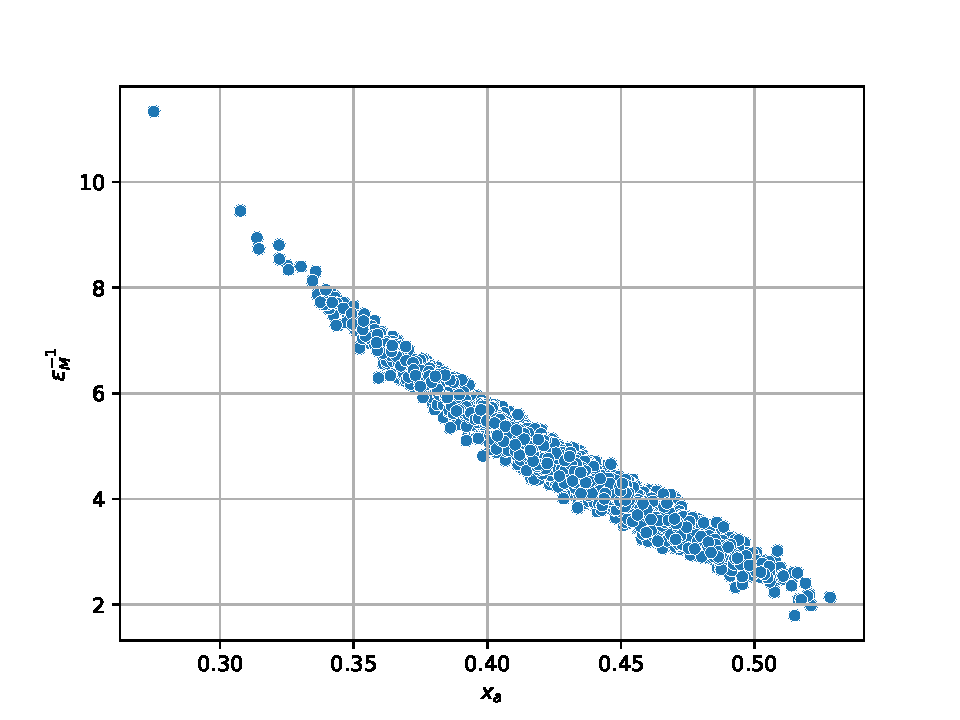
\includegraphics[width=0.49\textwidth]{figures/elasticity_vs_xa.pdf}
% %     \caption{Ergodic distribution of the macro price impact}
% %     \label{fig:price-impact-dist}
% % \end{figure}


% \subsection{Quantitative results}

% \paragraph{Numerical solution.} To assess the model's quantitative implications, we rely on a global solution method instead of the perturbation approach described in Section~\ref{sec:elasticity}.
% A method able to handle dimensional state spaces is necessary, as we have a total of $J+1$ state variables, and a total of $J = 6$ active sectors.  
% We adopt the neural-networks based method of \citet{duarte2024machine}. 
% We discuss the solution method in more detail in the appendix. 

% Figure~\ref{fig:results-model} plots the consumption-wealth ratio, dividend yield, interest rate, and price of risk as a function of the wealth share of active agents.
% \begin{figure}[t]
%     \centering
%     \subfloat{\resizebox{0.5\textwidth}{!}{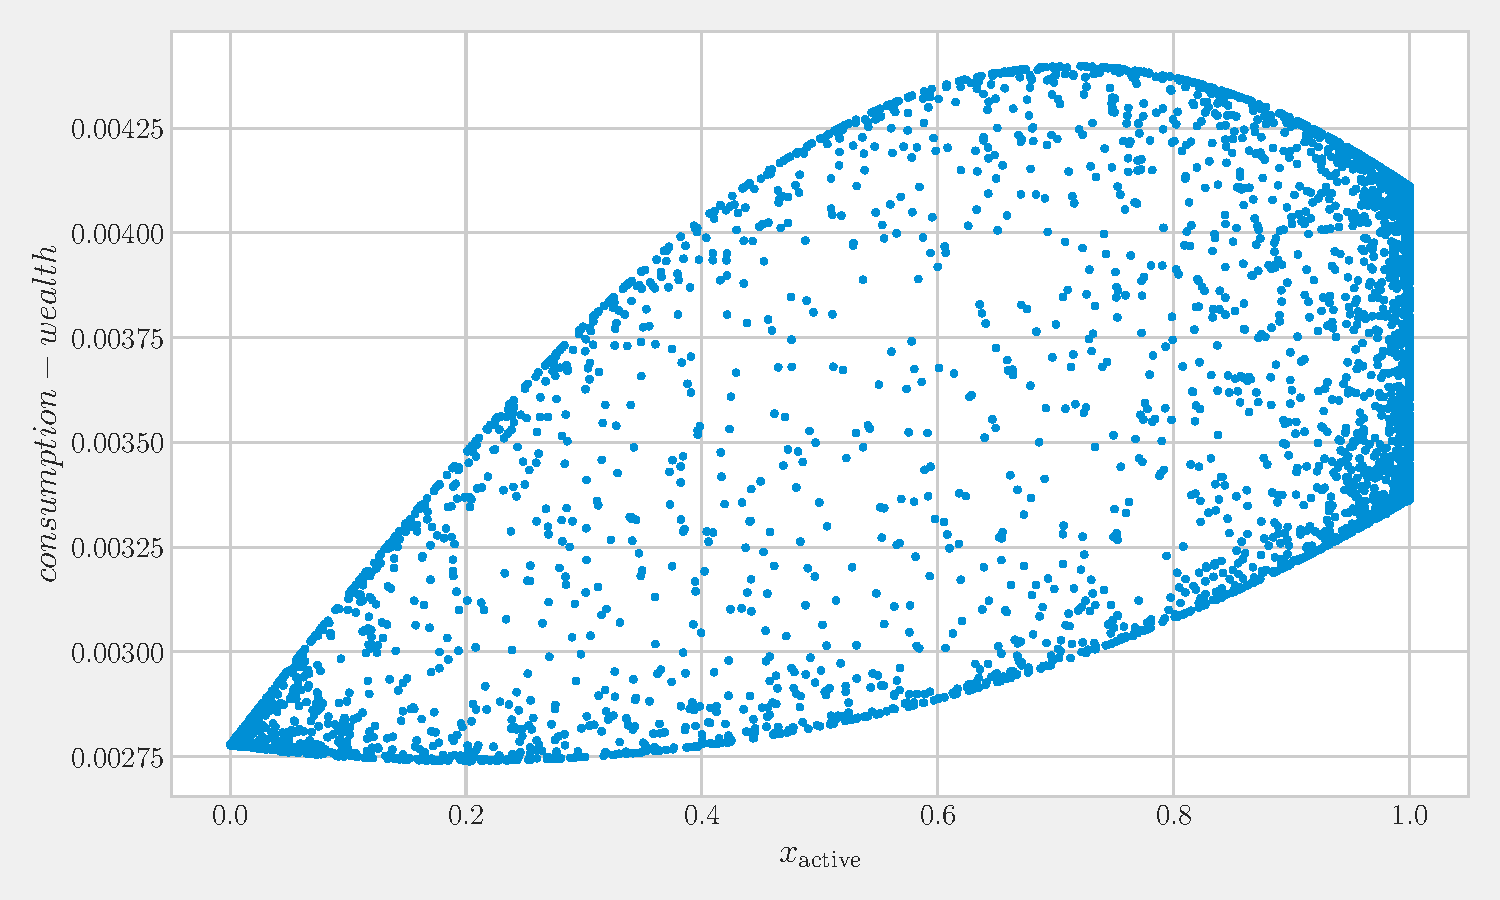
\includegraphics{figures/victor/c0.pdf}}}
%     \subfloat{\resizebox{0.5\textwidth}{!}{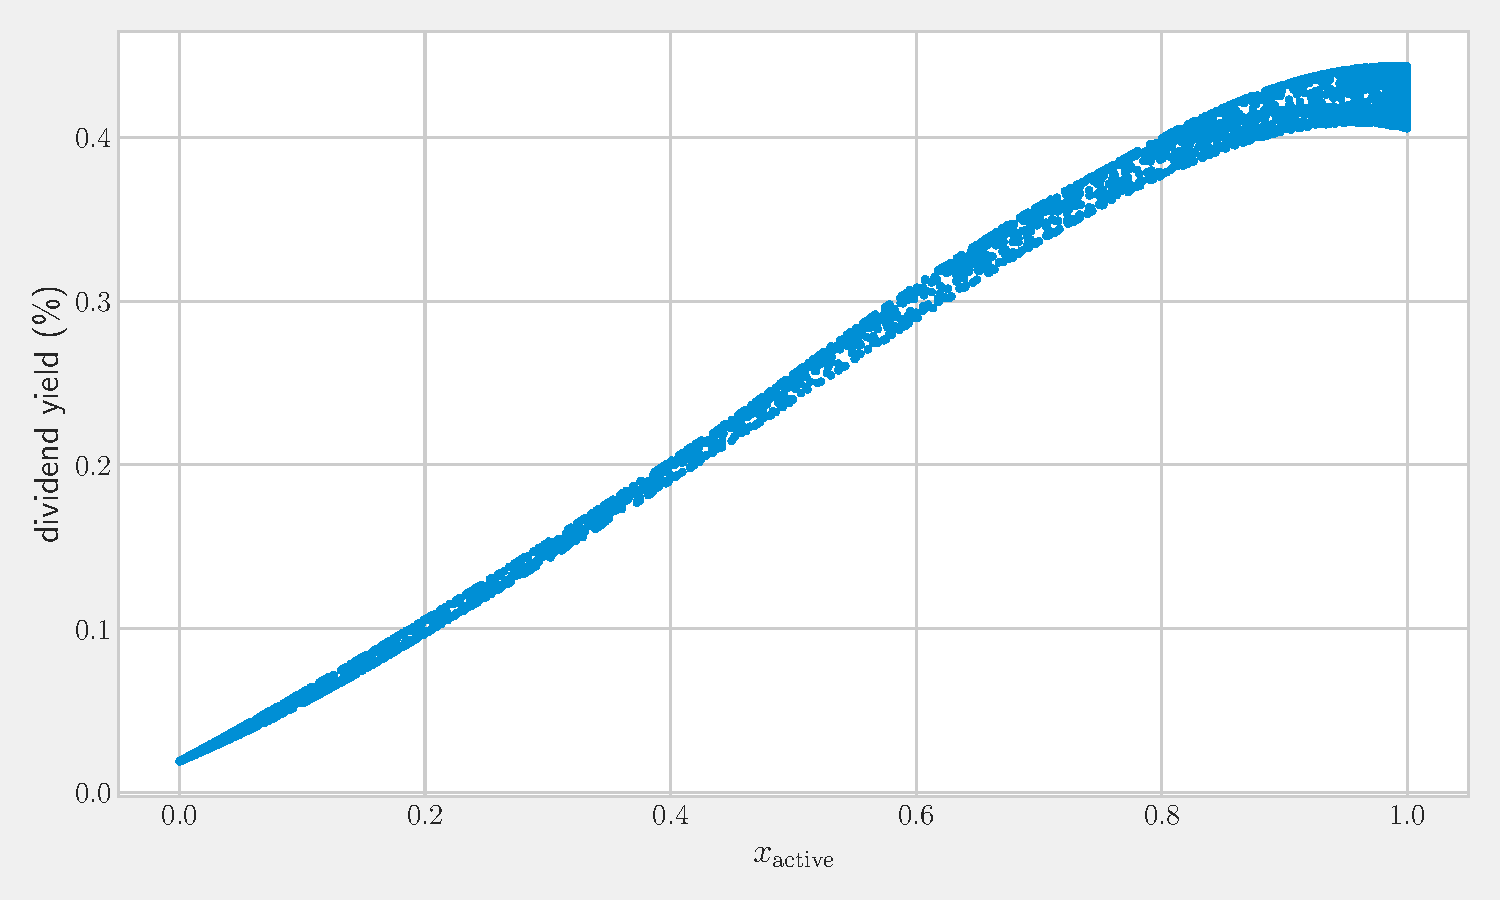
\includegraphics{figures/victor/y.pdf}}}\\
%     \subfloat{\resizebox{0.5\textwidth}{!}{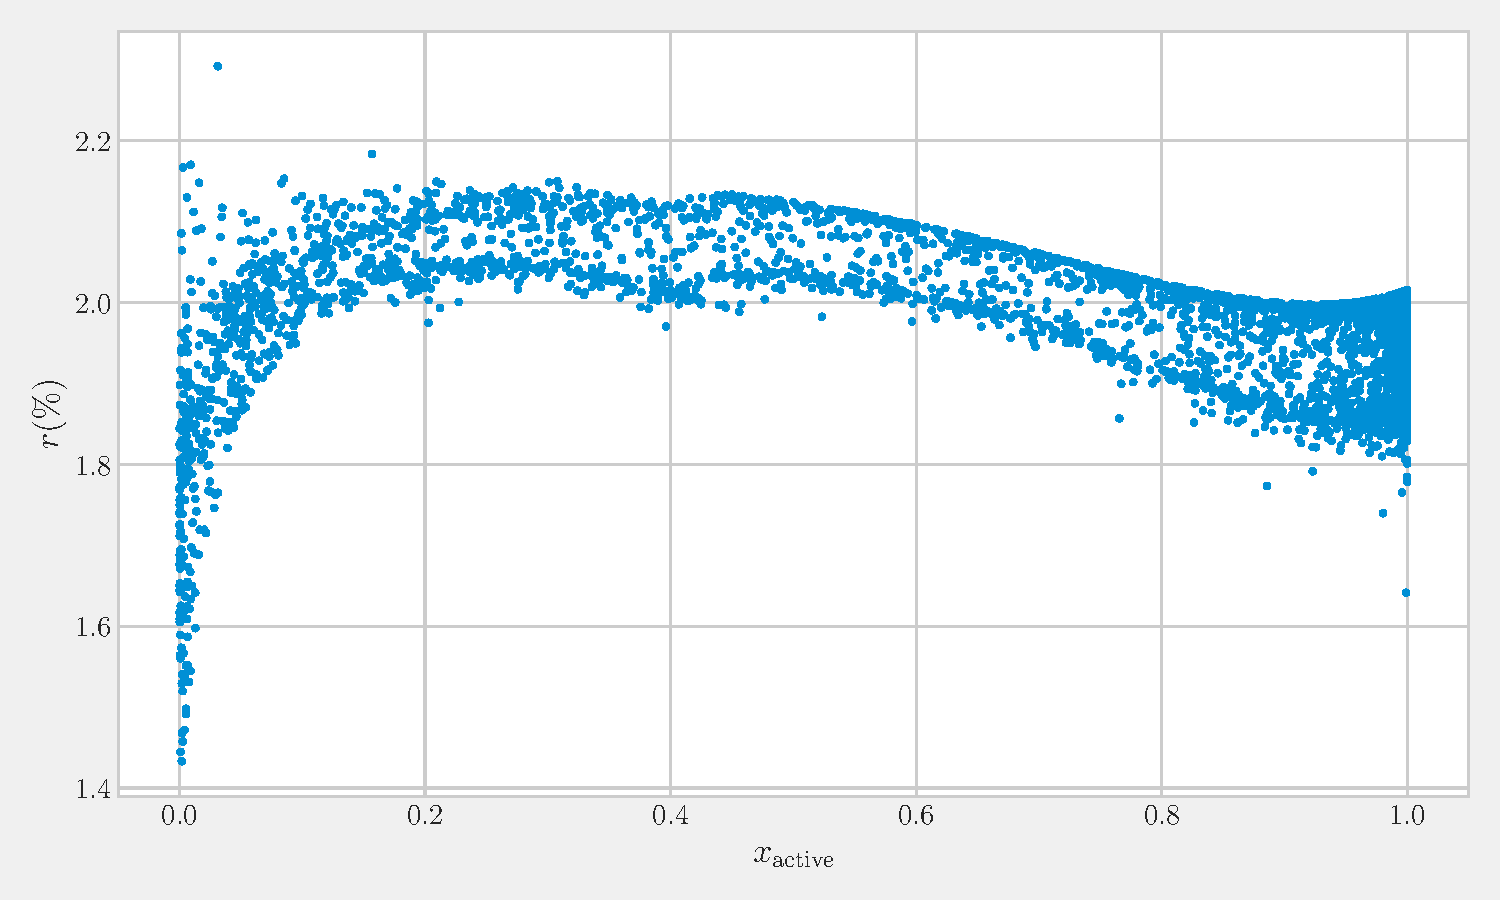
\includegraphics{figures/victor/r.pdf}}}
%     \subfloat{\resizebox{0.5\textwidth}{!}{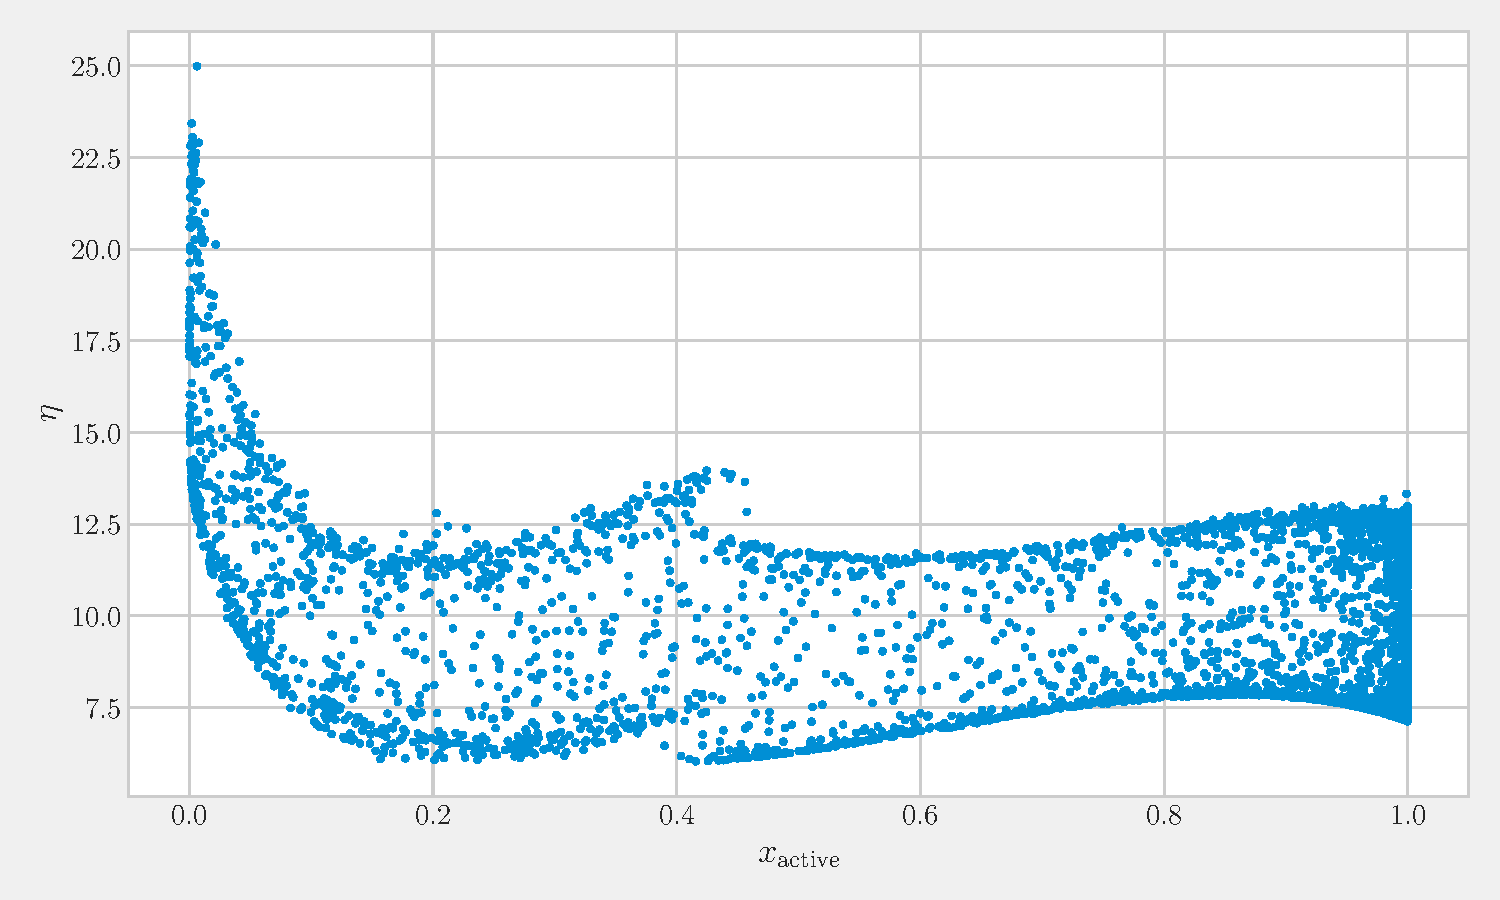
\includegraphics{figures/victor/eta.pdf}}}
%     \vspace{2mm}
%     \caption{Model results. This figure plots the consumption-wealth ratio, dividend yield, interest rate, and price of risk as a function of the wealth share of active agents.}\label{fig:results-model}
% \end{figure}

% Figure~\ref{fig:price-imapct-model} displays the price impact in the left panel and the aggregate elasticity (i.e., its inverse) in the right panel. We see that the price impact is comparable with the solution obtained using the global perturbation method in Section~\ref{sec:elasticity}.
% \begin{figure}[t]
%     \centering
%     \subfloat{\resizebox{0.5\textwidth}{!}{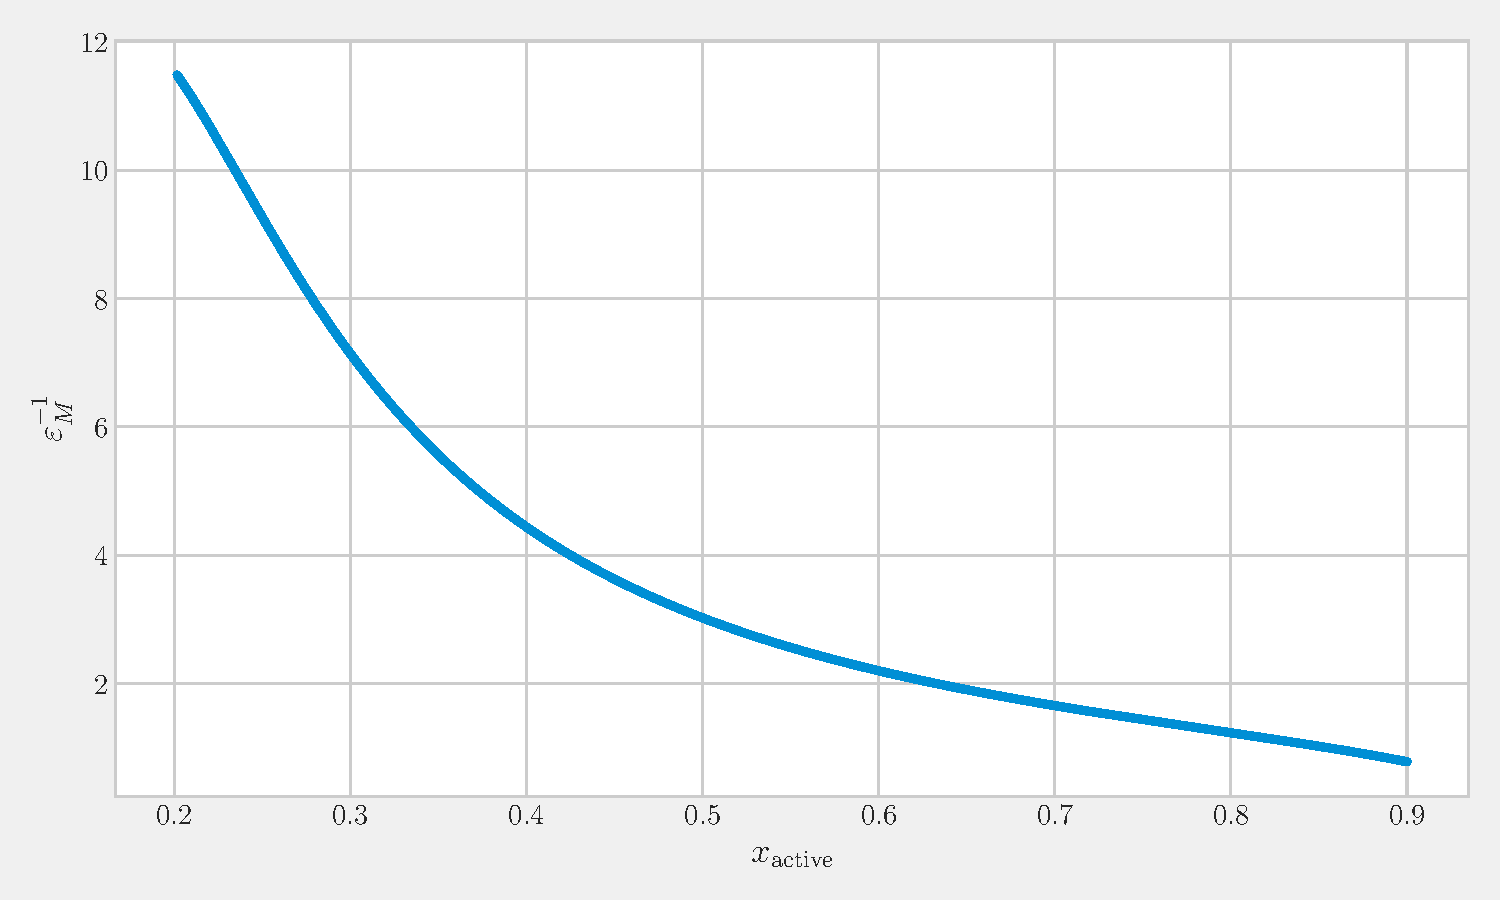
\includegraphics{figures/victor/price_impact.pdf}}}
%     \subfloat{\resizebox{0.5\textwidth}{!}{
\includegraphics{figures/victor/elasticity.pdf}}}
%     \vspace{2mm}
%     \caption{Price impact and aggregate elasticity.\\ The left panel plots the price impact and the right panel plots the aggregate elasticity.}\label{fig:price-imapct-model}
% \end{figure}
\section{Quantitative Implications}

In this section, we turn to the quantitative implications of the model described in Section~\ref{sec:model}. We begin by describing our calibration strategy before presenting numerical results.  

\subsection{Calibration strategy}

To calibrate the model, we process Flow of Funds (FoF) data to construct $J=6$ major sectors: household mutual fund holdings, household non-mutual fund holdings, hedge funds, broker-dealers (L.130), the rest of the world (L.133), and the insurance-pension sector. Figure~\ref{fig:sectors} plots the fraction of the U.S. stock market held by each of these sectors since 2012, the year when hedge fund holdings became separately available in the FoF. The legend reports the average fraction held by each sector. Households are the largest holders, accounting for 17.3\% of the market through mutual funds and 43.3\% through other vehicles. Foreign investors and the insurance-pension sector hold 17.5\% and 17.3\%, respectively. Hedge funds and broker-dealers are comparatively small, with average holdings of 5.8\% and 0.5\%, consistent with Figure~1 in \citet{koijen2024investors}.  

\begin{figure}[t]
    \centering
    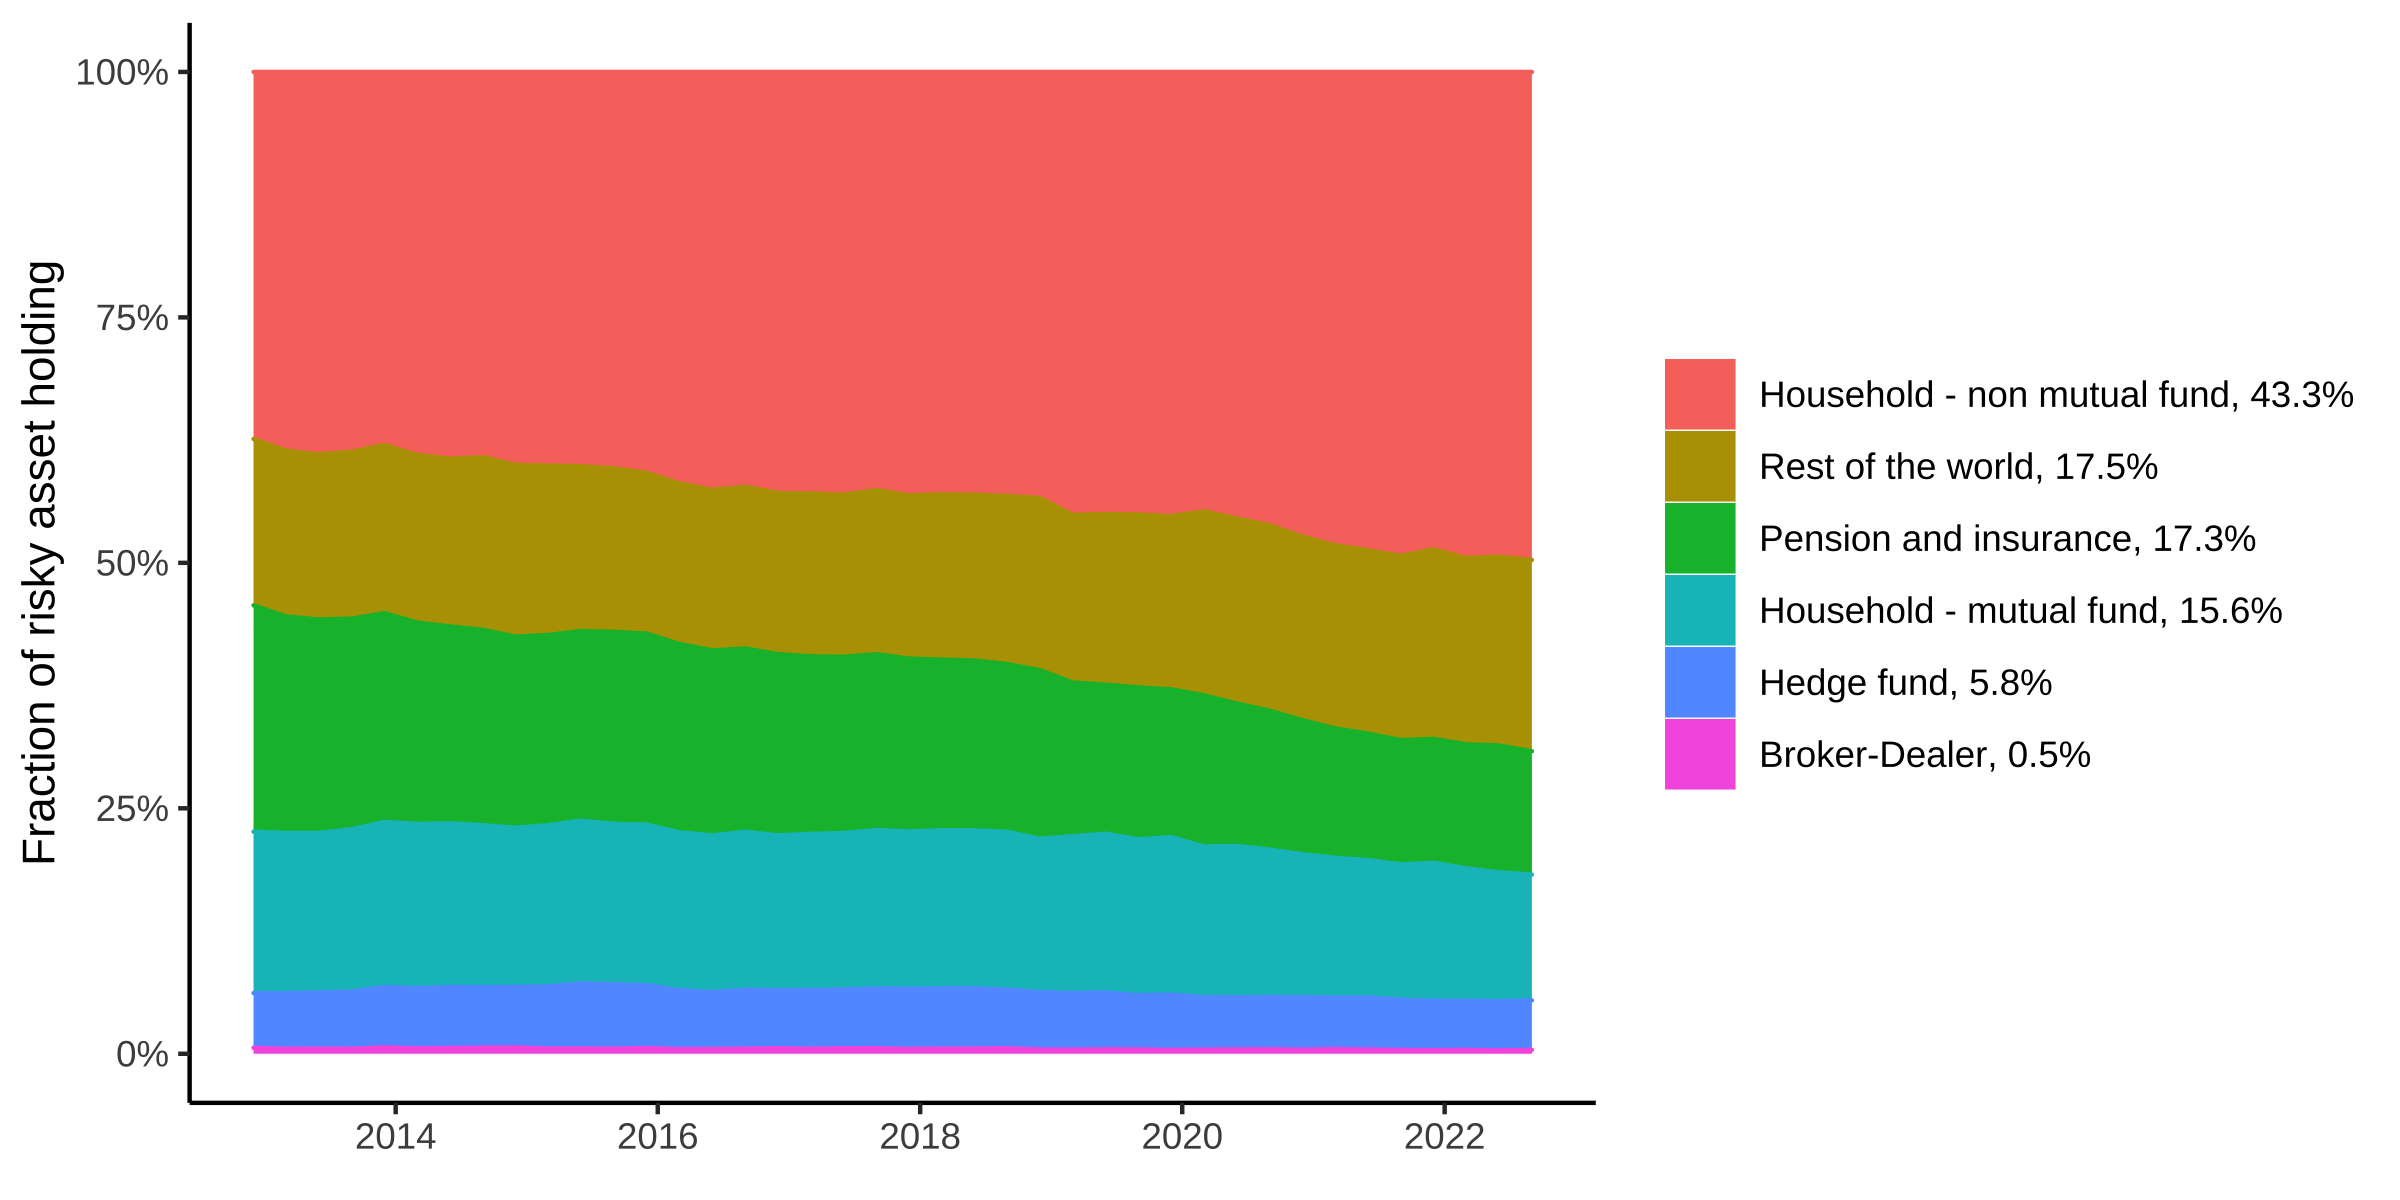
\includegraphics[width=0.9\linewidth]{figures/break_down_of_holdings.png}
    \caption{Fraction of stock market held by different sectors from 2012 to 2022. The average fraction held is reported in the legend. Source: Flow of Funds.}
    \label{fig:sectors}
\end{figure}

We exclude sectors with negligible stock market exposure, such as nonfinancial business (L.102), general government (L.105), the monetary authority (L.109), private depository institutions (L.110), money market funds (L.121), government-sponsored enterprises (L.125), agency- and GSE-backed mortgage pools (L.126), asset-backed security issuers (L.127), finance companies (L.128), REITs (L.129), holding companies (L.131), and other financial businesses (L.132). We then aggregate pass-through sectors back to their ultimate end users. For example, closed-end funds (L.123) and exchange-traded funds (L.124) are consolidated into the household (L.101) balance sheet, while mutual funds (L.122) are allocated across end investors based on the FOF breakdown. Defined contribution pensions (Tables L.118.c, L.119.c, and L.120.c) are also aggregated into the household sector.  

We separately construct the hedge fund sector, since both households (L.101) and foreign investors (L.133) include hedge funds in their reported holdings. Domestic hedge funds are identified from Table B.101.f, while foreign hedge funds are obtained from the Enhanced Financial Accounts. We subtract hedge fund holdings from both the household and foreign sectors and treat them as a distinct category. Finally, we combine the remaining insurance and pension subsectors, including property-casualty insurance (L.115), life insurance (L.116), and defined benefit pensions and retirement plans (L.118.b, L.119.b, L.120.b).  

We assign sectoral masses $\omega_j$ and risk aversion coefficients $\gamma_j$ to match two sets of moments. First, average sectoral wealth shares are calibrated to match the empirical distribution of stock market holdings. Second, we match sectoral betas from time-series regressions of risky asset holdings on aggregate risky asset supply. These regression coefficients provide an empirical analog to the model-implied relationship between sectoral and aggregate risky positions.  

A key parameter in the calibration is the average passive portfolio share, $\overline{\alpha}$. Estimates in the literature vary widely. \citet{chinco2024passive} infer a passive share of about one third from index reconstitution events, while \citet{koijen2024investors} report a much higher estimate of roughly two thirds in 2016Q4, based on measures of active share \citep{cremers2009active}. We calibrate the passive share by aggregating total passive wealth and dividing by total risky holdings.  

The process for passive demand is modeled as the exogenous CIR process in Equation~\eqref{eq:alpha_p_process}. Its parameters are calibrated as follows. The mean of the process, $\overline{\alpha}$, is chosen to match the average passive portfolio share described above. The volatility $\sigma_p$ is disciplined by observed fluctuations in equity flows, which we measure by scaling quarterly flows by lagged market capitalization, following Appendix D3 of \citet{gabaix2020search}. We use indirect inference to align model-implied aggregate flows with those in the data (blue line, left panel of Figure~\ref{fig:facts-vol-flow}), in line with their approach. The persistence parameter $\theta_p$ is informed by evidence on household portfolio inertia. \citet{brunnermeier2008wealth} document substantial inertia using PSID data, finding that household portfolios change little absent major events, consistent with slow rebalancing. Their regression analysis suggests an inertia coefficient near 0.75, indicating strong persistence.\footnote{Relatedly, \citet{parker2023retail} show that the adoption of target-date funds has contributed to highly stable household portfolio shares.} Finally, we calibrate the correlation between passive flow shocks and aggregate shocks by regressing quarterly flows (again, blue line in the left panel of Figure~\ref{fig:facts-vol-flow}) on aggregate market returns, with the estimated beta providing the implied correlation.  

The parameter values are summarized in Table~\ref{tab:calib}.  

\begin{table}[!t]    
    \captionsetup{font=normalsize,labelfont=bf,skip=2pt,labelsep=period}
	\caption{\textbf{Parameter values}}
	\caption*{\footnotesize{This table reports the parameter values used in calibrating the model.}}
    \vspace{2mm}
    \label{tab:calib}
    \centering
    \resizebox{.65\linewidth}{!}{\begin{tabular}{llc}
	\toprule	
	& Parameter & Choice  \\
	\midrule 
	&\small \emph{Preferences \& distribution}  & \\
	\midrule		
	$\psi$         & EIS & 1.50   \\
	$\gamma_0$     & Risk aversion of passive investors               & 10.86    \\
	$\gamma_j$     & Risk aversion of constrained investors                & 6.15 \\
    $\gamma_j$     & Risk aversion of unconstrained investors                & 25.52 \\ 
	$\rho$         & Effective discount rate                  & 0.01 \\
    $\kappa$       & Agent turnover rate                      & 0.10 \\
    $\omega_0$    & Share of passive agents                & 0.50 \\
    $\omega_1$    & Share of unconstrained agents                & 0.25 \\
	$\omega_2$    & Share of constrained agents                & 0.25 \\
	\midrule 
	& \small \emph{Technology}  & \\
	\midrule 
	$\mu$          & Endowment growth rate                    & 0.018  \\
	$\|\sigma\|$       & Endowment volatility                     & 0.033  \\
    $\|\sigma_s\|$     & Dividend share volatility                & 0.11 \\ 
    $\bar{s}$      & Mean dividend share                      & 0.60 \\ 
    $\kappa_s$     & Mean reversion of dividend share         & 0.09 \\
	$\nu_s$     & Corr. of dividend share and fundamental shock         & 0.30 \\
	\midrule 
	&\small \emph{Passive demand}&  \\
	\midrule
	$\overline{\alpha}$ & Mean &  0.52	\\
    $\theta_p$              & Mean reversion parameter  &  0.75 	\\
    $\sigma_p$             & Passive demand shock exposures &  0.02	\\
    $\nu_p$                  & Corr. of passive demand and fundamental shock & 0.50 \\ 

	\midrule
	& \small \emph{Leverage constraints}  & \\
	\midrule 
	$\overline{\sigma}$ & Tightness of the leverage constraint &  0.11	\\
	\bottomrule
\end{tabular}

%γ_vec=[10., 9.368, 4.925, 3.212, 1.552],
%ψ=2.5,
%ρ_=0.02,
%μ=0.022,
%σ=0.035,
%θp=0.69,
%σp0_=0.1,
%σp1_=0.02,
%σ_hat=0.02,
%κ_=0.05,
%α_=.1,
%ω=0.90713995, 0.02905808, 0.02313385, 0.02031372, 0.02035439}
\end{table}

\subsection{Quantitative results}

To evaluate the quantitative implications of the model, we solve the full dynamic system numerically rather than relying on the perturbation approach of Section~\ref{sec:elasticity}. A global solution method is necessary given the dimensionality of the state space, which includes $J+1$ state variables corresponding to one passive sector and six active sectors. We adopt the neural network-based method of \citet{duarte2024machine}, which is well suited for high-dimensional problems. Details of the solution method are provided in the appendix.  

% Figure~\ref{fig:results-model} plots the consumption-wealth ratio, dividend yield, interest rate, and price of risk as functions of the wealth share of active agents. These results highlight how sectoral wealth distribution shapes equilibrium outcomes.  

% \begin{figure}[t]
%     \centering
%     \subfloat{\resizebox{0.5\textwidth}{!}{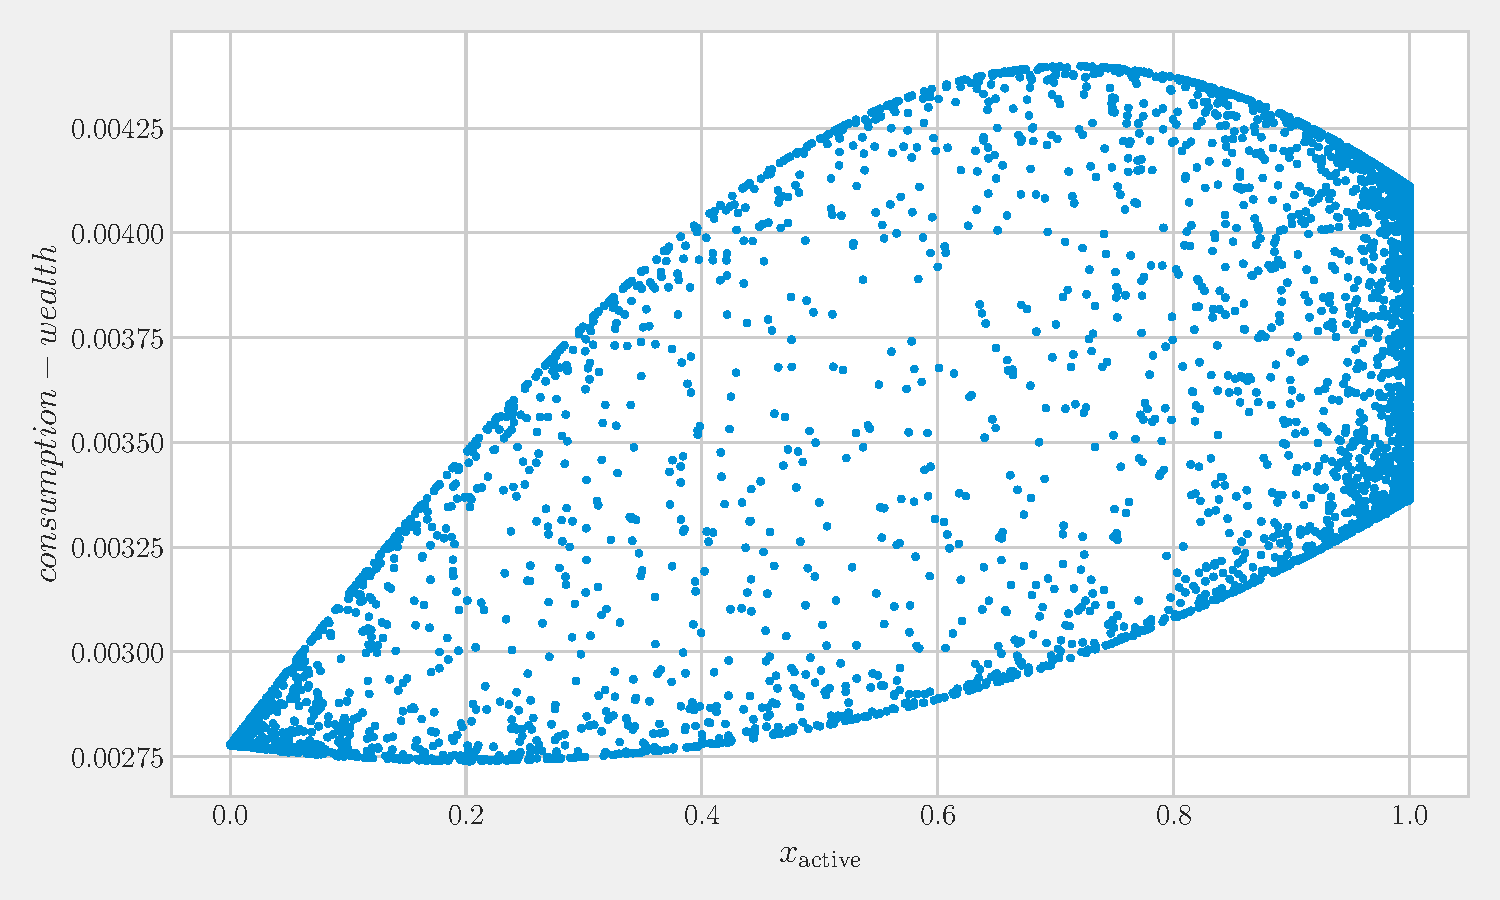
\includegraphics{figures/victor/c0.pdf}}}
%     \subfloat{\resizebox{0.5\textwidth}{!}{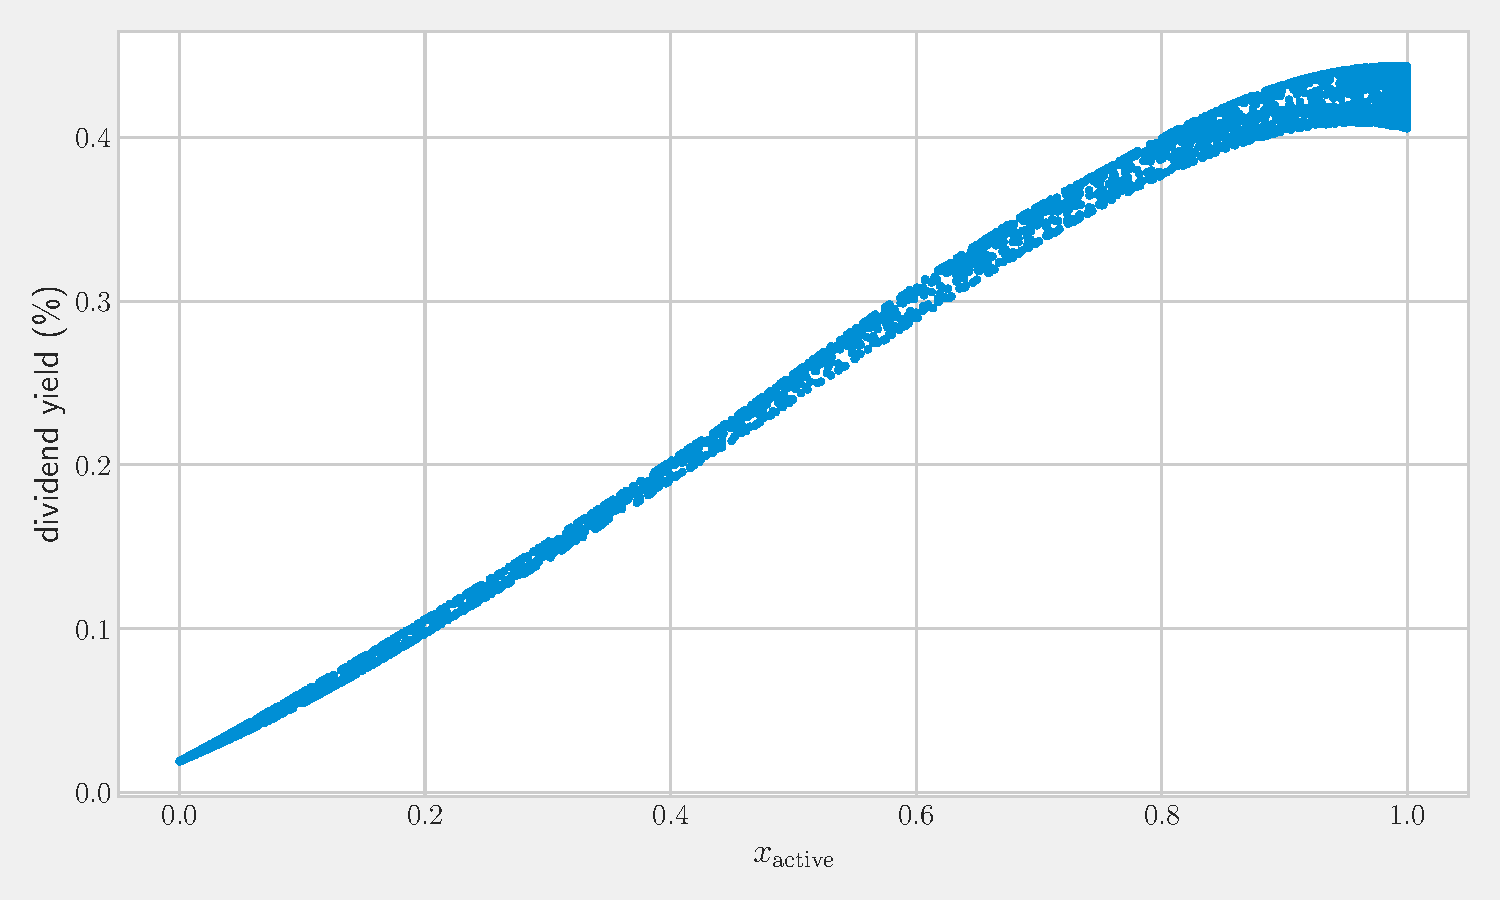
\includegraphics{figures/victor/y.pdf}}}\\
%     \subfloat{\resizebox{0.5\textwidth}{!}{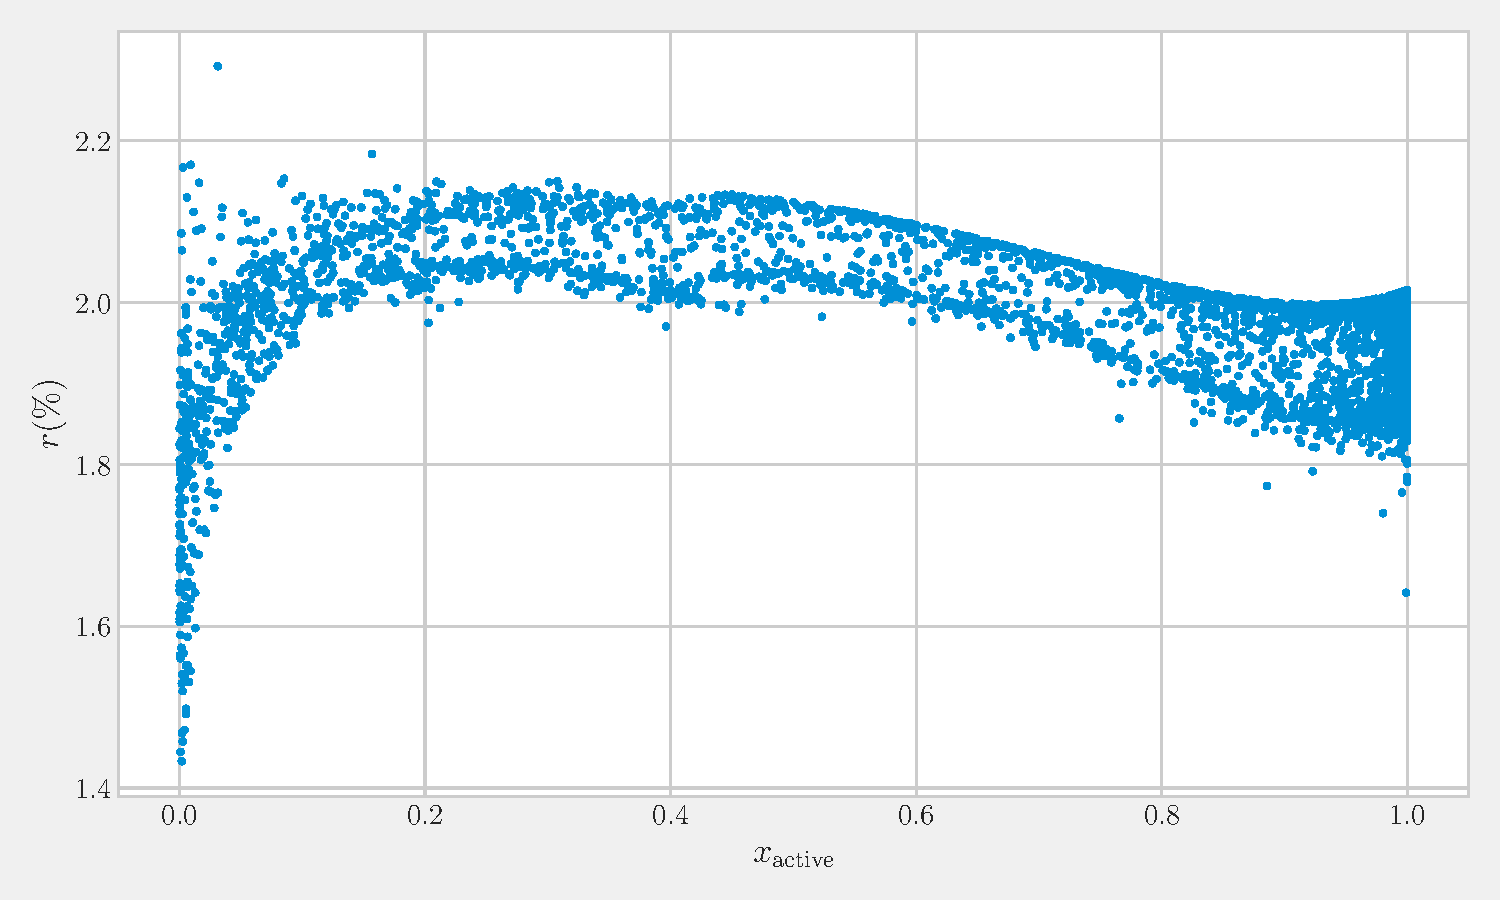
\includegraphics{figures/victor/r.pdf}}}
%     \subfloat{\resizebox{0.5\textwidth}{!}{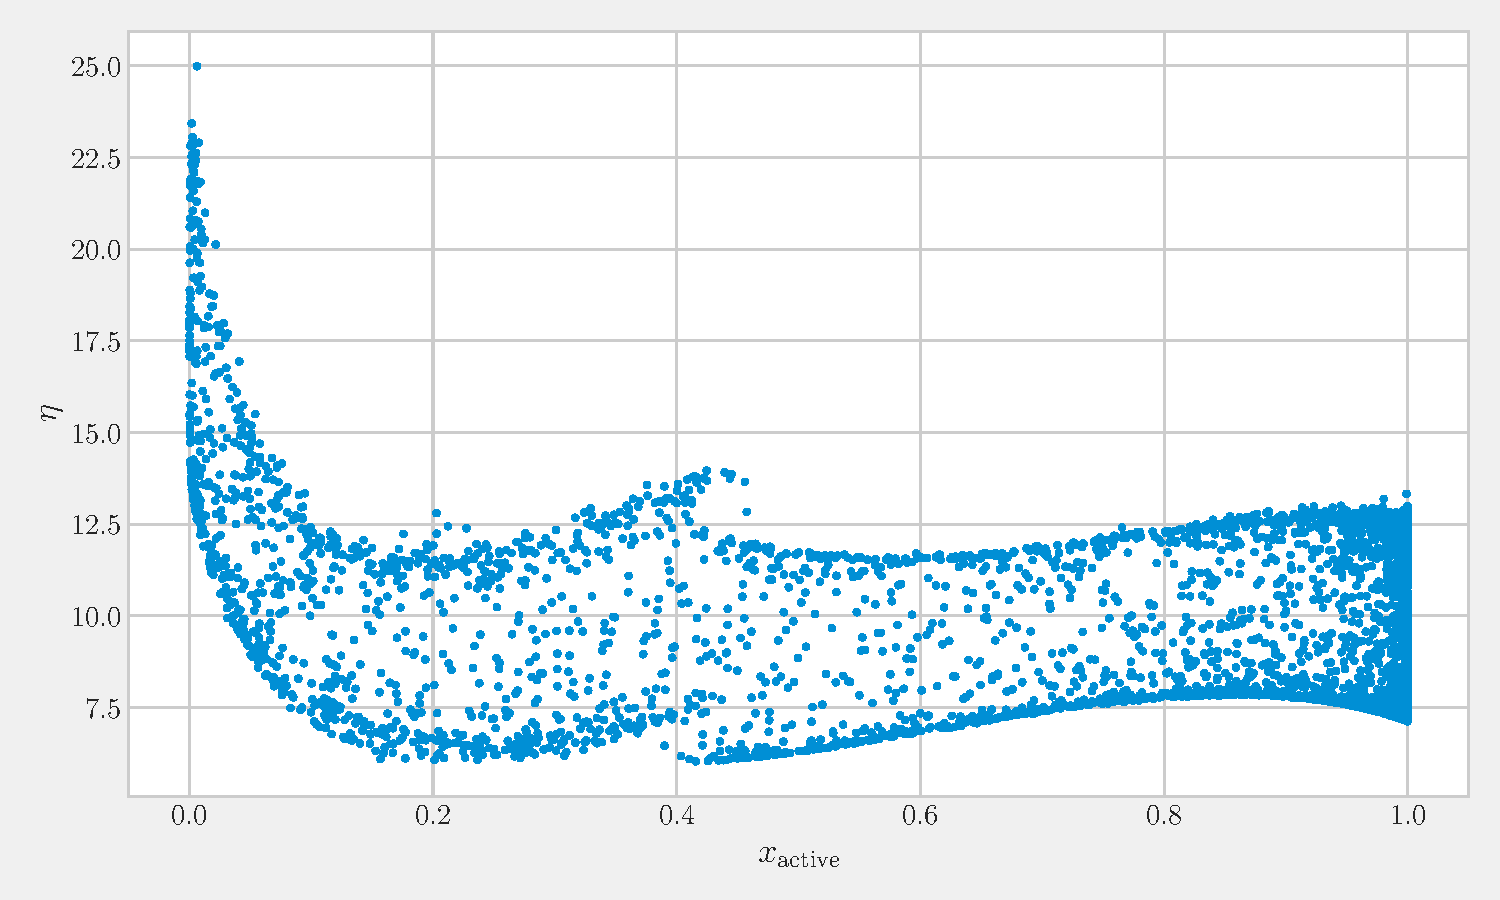
\includegraphics{figures/victor/eta.pdf}}}
%     \vspace{2mm}
%     \caption{Model results. The consumption–wealth ratio, dividend yield, interest rate, and price of risk as functions of the wealth share of active agents.}\label{fig:results-model}
% \end{figure}

% Figure~\ref{fig:price-imapct-model} shows the model-implied price impact (left panel) and aggregate elasticity, defined as its inverse (right panel). The estimates are broadly consistent with those obtained using the global perturbation method of Section~\ref{sec:elasticity}, reinforcing the robustness of the main results.  

% \begin{figure}[t]
%     \centering
%     \subfloat{\resizebox{0.5\textwidth}{!}{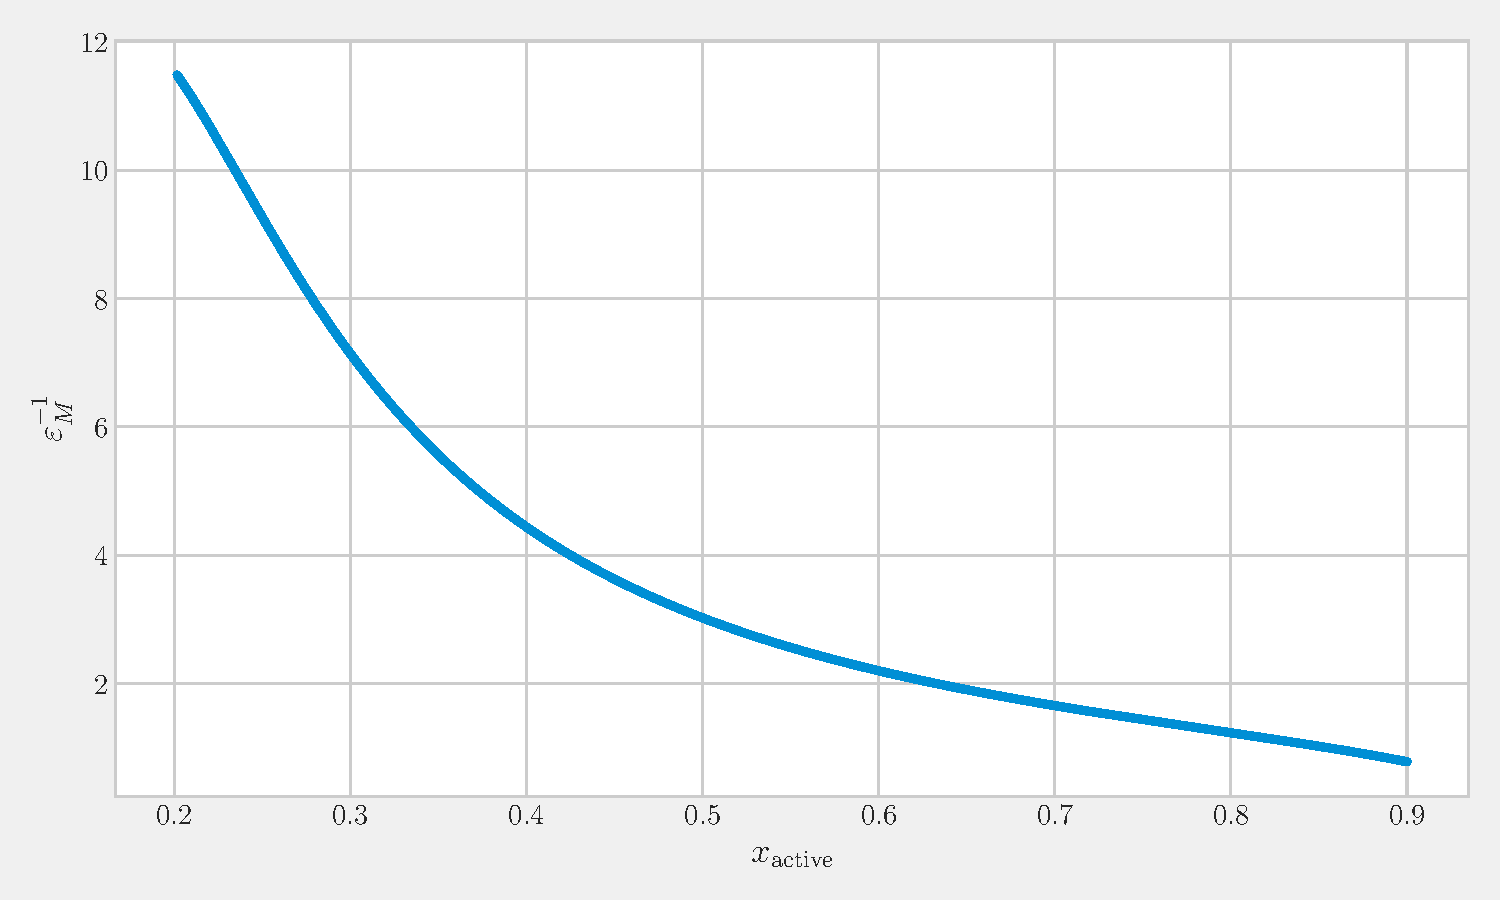
\includegraphics{figures/victor/price_impact.pdf}}}
%     \subfloat{\resizebox{0.5\textwidth}{!}{
\includegraphics{figures/victor/elasticity.pdf}}}
%     \vspace{2mm}
%     \caption{Price impact and aggregate elasticity. The left panel plots the price impact; the right panel plots the corresponding aggregate elasticity.}\label{fig:price-imapct-model}
% \end{figure}
